\PassOptionsToPackage{unicode=true}{hyperref} % options for packages loaded elsewhere
\PassOptionsToPackage{hyphens}{url}
%
\documentclass[]{scrartcl}
\usepackage{lmodern}
\usepackage{amssymb,amsmath}
\usepackage{ifxetex,ifluatex}
\usepackage{fixltx2e} % provides \textsubscript
\ifnum 0\ifxetex 1\fi\ifluatex 1\fi=0 % if pdftex
  \usepackage[T1]{fontenc}
  \usepackage[utf8]{inputenc}
  \usepackage{textcomp} % provides euro and other symbols
\else % if luatex or xelatex
  \usepackage{unicode-math}
  \defaultfontfeatures{Ligatures=TeX,Scale=MatchLowercase}
\fi
% use upquote if available, for straight quotes in verbatim environments
\IfFileExists{upquote.sty}{\usepackage{upquote}}{}
% use microtype if available
\IfFileExists{microtype.sty}{%
\usepackage[]{microtype}
\UseMicrotypeSet[protrusion]{basicmath} % disable protrusion for tt fonts
}{}
\IfFileExists{parskip.sty}{%
\usepackage{parskip}
}{% else
\setlength{\parindent}{0pt}
\setlength{\parskip}{6pt plus 2pt minus 1pt}
}
\usepackage{hyperref}
\hypersetup{
            pdftitle={Devoir Maison de mathématiques},
            pdfauthor={Antonin Peronnet, Benoit Leroux, Oscar Plaisant},
            pdfborder={0 0 0},
            breaklinks=true}
\urlstyle{same}  % don't use monospace font for urls
\usepackage{color}
\usepackage{fancyvrb}
\newcommand{\VerbBar}{|}
\newcommand{\VERB}{\Verb[commandchars=\\\{\}]}
\DefineVerbatimEnvironment{Highlighting}{Verbatim}{commandchars=\\\{\}}
% Add ',fontsize=\small' for more characters per line
\newenvironment{Shaded}{}{}
\newcommand{\AlertTok}[1]{\textcolor[rgb]{1.00,0.00,0.00}{\textbf{#1}}}
\newcommand{\AnnotationTok}[1]{\textcolor[rgb]{0.38,0.63,0.69}{\textbf{\textit{#1}}}}
\newcommand{\AttributeTok}[1]{\textcolor[rgb]{0.49,0.56,0.16}{#1}}
\newcommand{\BaseNTok}[1]{\textcolor[rgb]{0.25,0.63,0.44}{#1}}
\newcommand{\BuiltInTok}[1]{#1}
\newcommand{\CharTok}[1]{\textcolor[rgb]{0.25,0.44,0.63}{#1}}
\newcommand{\CommentTok}[1]{\textcolor[rgb]{0.38,0.63,0.69}{\textit{#1}}}
\newcommand{\CommentVarTok}[1]{\textcolor[rgb]{0.38,0.63,0.69}{\textbf{\textit{#1}}}}
\newcommand{\ConstantTok}[1]{\textcolor[rgb]{0.53,0.00,0.00}{#1}}
\newcommand{\ControlFlowTok}[1]{\textcolor[rgb]{0.00,0.44,0.13}{\textbf{#1}}}
\newcommand{\DataTypeTok}[1]{\textcolor[rgb]{0.56,0.13,0.00}{#1}}
\newcommand{\DecValTok}[1]{\textcolor[rgb]{0.25,0.63,0.44}{#1}}
\newcommand{\DocumentationTok}[1]{\textcolor[rgb]{0.73,0.13,0.13}{\textit{#1}}}
\newcommand{\ErrorTok}[1]{\textcolor[rgb]{1.00,0.00,0.00}{\textbf{#1}}}
\newcommand{\ExtensionTok}[1]{#1}
\newcommand{\FloatTok}[1]{\textcolor[rgb]{0.25,0.63,0.44}{#1}}
\newcommand{\FunctionTok}[1]{\textcolor[rgb]{0.02,0.16,0.49}{#1}}
\newcommand{\ImportTok}[1]{#1}
\newcommand{\InformationTok}[1]{\textcolor[rgb]{0.38,0.63,0.69}{\textbf{\textit{#1}}}}
\newcommand{\KeywordTok}[1]{\textcolor[rgb]{0.00,0.44,0.13}{\textbf{#1}}}
\newcommand{\NormalTok}[1]{#1}
\newcommand{\OperatorTok}[1]{\textcolor[rgb]{0.40,0.40,0.40}{#1}}
\newcommand{\OtherTok}[1]{\textcolor[rgb]{0.00,0.44,0.13}{#1}}
\newcommand{\PreprocessorTok}[1]{\textcolor[rgb]{0.74,0.48,0.00}{#1}}
\newcommand{\RegionMarkerTok}[1]{#1}
\newcommand{\SpecialCharTok}[1]{\textcolor[rgb]{0.25,0.44,0.63}{#1}}
\newcommand{\SpecialStringTok}[1]{\textcolor[rgb]{0.73,0.40,0.53}{#1}}
\newcommand{\StringTok}[1]{\textcolor[rgb]{0.25,0.44,0.63}{#1}}
\newcommand{\VariableTok}[1]{\textcolor[rgb]{0.10,0.09,0.49}{#1}}
\newcommand{\VerbatimStringTok}[1]{\textcolor[rgb]{0.25,0.44,0.63}{#1}}
\newcommand{\WarningTok}[1]{\textcolor[rgb]{0.38,0.63,0.69}{\textbf{\textit{#1}}}}
\usepackage{longtable,booktabs}
% Fix footnotes in tables (requires footnote package)
\IfFileExists{footnote.sty}{\usepackage{footnote}\makesavenoteenv{longtable}}{}
\setlength{\emergencystretch}{3em}  % prevent overfull lines
\providecommand{\tightlist}{%
  \setlength{\itemsep}{0pt}\setlength{\parskip}{0pt}}
\setcounter{secnumdepth}{0}
% Redefines (sub)paragraphs to behave more like sections
\ifx\paragraph\undefined\else
\let\oldparagraph\paragraph
\renewcommand{\paragraph}[1]{\oldparagraph{#1}\mbox{}}
\fi
\ifx\subparagraph\undefined\else
\let\oldsubparagraph\subparagraph
\renewcommand{\subparagraph}[1]{\oldsubparagraph{#1}\mbox{}}
\fi

% set default figure placement to htbp
\makeatletter
\def\fps@figure{htbp}
\makeatother

\usepackage[utf8]{inputenc}
\usepackage[T1]{fontenc}
\usepackage[french]{babel}

\usepackage[left=1.2cm, right=1.2cm, top=2cm, bottom=2.5cm]{geometry}

\usepackage{amsmath, amsfonts, amssymb}

\usepackage{xcolor}
\usepackage{enumitem}
\usepackage{fancyhdr}
\usepackage{sectsty}
\usepackage{graphicx}
\usepackage{euler}

\pagestyle{fancy}

\renewcommand{\headrulewidth}{0pt}
\fancyhead[L]{}
\fancyhead[C]{}
\fancyhead[R]{}

\renewcommand{\footrulewidth}{1pt}
\fancyfoot[L]{Antonin\;Peronnet,\;Benoit\;Leroux,\;Oscar\;Plaisant}
\fancyfoot[C]{\thepage/13}
\fancyfoot[R]{\.\.\text{DM N}$^\circ3$}

\renewcommand{\frac}[2]{\dfrac{#1}{#2}}

\sectionfont{\Huge}
\subsectionfont{\huge}
\subsubsectionfont{\Large}
\paragraphfont{\large}

\newcommand{\br}{\vspace*{2cm}}

\title{\huge Devoir Maison de mathématiques}
\author{Antonin Peronnet, Benoit Leroux, Oscar Plaisant}
\date{}

\begin{document}
\maketitle

\hypertarget{exercice-1}{%
\section{Exercice 1 :}\label{exercice-1}}

\(u_0 = 3\)

\(u_1 = 6\)

\(u_{n+2} = \dfrac{5}{4}u_{n+1} -\dfrac{1}{4}u_n\)

\hypertarget{partie-a}{%
\subsection{Partie A}\label{partie-a}}

\hypertarget{donner-une-formule-qui-saisie-dans-la-cellule-b4-puis-recopiuxe9e-vers-le-bas-permet-dobtenir-les-valeurs-de-la-suite-u_n-dans-la-colonne-b.}{%
\subsubsection{\texorpdfstring{1. Donner une formule qui, saisie dans la
cellule B4, puis recopiée vers le bas, permet d'obtenir les valeurs de
la suite \((u_n)\) dans la colonne
B.}{1. Donner une formule qui, saisie dans la cellule B4, puis recopiée vers le bas, permet d'obtenir les valeurs de la suite (u\_n) dans la colonne B.}}\label{donner-une-formule-qui-saisie-dans-la-cellule-b4-puis-recopiuxe9e-vers-le-bas-permet-dobtenir-les-valeurs-de-la-suite-u_n-dans-la-colonne-b.}}

La formule est ``=(5*B3/4) + (B2/4)''

\hypertarget{recopier-et-compluxe9ter-le-tableau-ci-dessus.-on-donnera-des-valeurs-approchuxe9es-uxe0-10---3-pruxe8s-deun-pour-n-allant-de-2-uxe0-5.}{%
\subsubsection{\texorpdfstring{2. Recopier et compléter le tableau
ci-dessus. On donnera des valeurs approchées à 10 - 3 près deun pour
\(n\) allant de 2 à
5.}{2. Recopier et compléter le tableau ci-dessus. On donnera des valeurs approchées à 10 - 3 près deun pour n allant de 2 à 5.}}\label{recopier-et-compluxe9ter-le-tableau-ci-dessus.-on-donnera-des-valeurs-approchuxe9es-uxe0-10---3-pruxe8s-deun-pour-n-allant-de-2-uxe0-5.}}

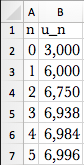
\includegraphics[scale=0.5]{images/tableur.png}

\hypertarget{que-peut-on-conjecturer-uxe0-propose-de-la-convergence-de-la-suite-u_n}{%
\subsubsection{\texorpdfstring{3. Que peut-on conjecturer à propose de
la convergence de la suite \((u_n)\)
?}{3. Que peut-on conjecturer à propose de la convergence de la suite (u\_n) ?}}\label{que-peut-on-conjecturer-uxe0-propose-de-la-convergence-de-la-suite-u_n}}

On peut conjecturer que la suite diverge vers \(+\infty\)

\hypertarget{partie-b}{%
\subsection{Partie B}\label{partie-b}}

\hypertarget{section}{%
\subsubsection{1.}\label{section}}

\hypertarget{a-duxe9montrer-que-v_n-est-une-suite-constante}{%
\paragraph{\texorpdfstring{a) Démontrer que \((v_n)\) est une suite
constante}{a) Démontrer que (v\_n) est une suite constante}}\label{a-duxe9montrer-que-v_n-est-une-suite-constante}}

\[
\begin{array}{rcl}
    v_n = u_{n+1} - \dfrac{1}{4}u_n & \iff & v_{n+1} = u_{n+2} + \dfrac{1}{4}u_{n+1}\\
        &\iff& v_{n+1} = \left(\dfrac{5}{4}u_{n+1} - \dfrac{1}{4}u_n\right) - \dfrac{1}{4}u_{n+1}\\
        &\iff& v_{n+1} = u_{n+1} - \dfrac{1}{4}u_{n+1}\\
        &\iff& v_{n+1} = v_n
\end{array}
\] Donc, la suite \((v_n)\) est constante. \#\#\#\# b) En déduire que,
pour tout \(n\in\mathbb{N}, u_{n+1} = \dfrac{1}{4}u_n + \dfrac{21}{4}\)

On sait que \[
\begin{array}{rcl}
    u_{n+1} &=& v_n + \dfrac{1}{4}u_n\\
            &=& v_0 + \dfrac{1}{4}u_n\\
            &=& \dfrac{21}{4} + \dfrac{1}{4}u_n\\ 
\end{array}
\]

\hypertarget{section-1}{%
\subsubsection{2.}\label{section-1}}

\hypertarget{a-en-utilisant-le-ruxe9sultat-de-la-question-1.b-montrer-par-ruxe9currence-que-forall-ninmathbbn-u_nleq-u_n1leq-15}{%
\paragraph{\texorpdfstring{a) En utilisant le résultat de la question
\textbf{1.b)}, montrer par récurrence que
\(\forall n\in\mathbb{N}, u_n\leq u_{n+1}\leq 15\)\textbackslash{}}{a) En utilisant le résultat de la question 1.b), montrer par récurrence que \textbackslash{}forall n\textbackslash{}in\textbackslash{}mathbb\{N\}, u\_n\textbackslash{}leq u\_\{n+1\}\textbackslash{}leq 15\textbackslash{}}}\label{a-en-utilisant-le-ruxe9sultat-de-la-question-1.b-montrer-par-ruxe9currence-que-forall-ninmathbbn-u_nleq-u_n1leq-15}}

On pose \(P\), la proposition : \(P_n \iff u_n\leq u_{n+1}\leq 15\)

\hypertarget{initialisation}{%
\subparagraph{Initialisation}\label{initialisation}}

\(P_0 \iff u_0 \leq u_1 \leq 15 \iff 3 \leq 6\leq 15\)

Donc, \(P_0\) est vraie.

\hypertarget{huxe9ruxe9dituxe9}{%
\subparagraph{Hérédité}\label{huxe9ruxe9dituxe9}}

On cherche à montrer que
\(\forall n\in\mathbb{N}, P_n\implies P_{n+1}\).

\[
\begin{array}{rcl}
    P_n &\iff& u_n \leq u_{n+1}\leq 15\\[2ex]
        &\iff& \dfrac{1}{4}u_n \leq \dfrac{1}{4}u_{n+1} \leq \dfrac{15}{4}\\[2ex]
        &\iff& \dfrac{1}{4}u_n + \dfrac{21}{4}u_n \leq \dfrac{1}{4}u_{n+1} + \dfrac{21}{4} \leq \dfrac{15}{4} + \dfrac{21}{4}\\[2ex]
        &\iff& u_{n+1} \leq u_{n+2} \leq 9\\[2ex]
        &\implies& u_{n+1} \leq u_{n+2} \leq 15
\end{array}
\]

On à donc bien \(P_n \implies P_{n+1}\)

\hypertarget{ruxe9currence}{%
\subparagraph{Récurrence}\label{ruxe9currence}}

puisque \(P_0 \wedge \forall n\in\mathbb{N}, P_n\implies P_{n+1}\), on
sait que \(\forall n\in\mathbb{N}, P_n\) b) En déduire que la suite
\((u_n)\) est une suite convergente.

La suite \((u_n)\) est strictement croissante et majorée par 15, on peut
donc dire qu'elle converge.

\hypertarget{section-2}{%
\subsubsection{3.}\label{section-2}}

\hypertarget{a-duxe9montrer-que-w_n-est-une-suite-guxe9omuxe9trique-dont-on-pruxe9cisera-le-premier-terme-et-la-raison}{%
\paragraph{\texorpdfstring{a) Démontrer que \((w_n)\) est une suite
géométrique dont on précisera le premier terme et la
raison}{a) Démontrer que (w\_n) est une suite géométrique dont on précisera le premier terme et la raison}}\label{a-duxe9montrer-que-w_n-est-une-suite-guxe9omuxe9trique-dont-on-pruxe9cisera-le-premier-terme-et-la-raison}}

On sait que :

\(w_n = u_n - 7\)

On peut donc en déduire que :

\(w_0=u_0-7=3-7=-4\)

Et que :

\[
\begin{array}{rcl}
    w_{n+1} &=& u_{n+1} - 7\\
            &=& \dfrac{u_n}{4} + \dfrac{21}{4} - \dfrac{28}{4}\\
            &=& \dfrac{u_n - 7}{4}\\
    w_{n+1} &=& \dfrac{1}{4}w_n
\end{array}
\]

On à donc :

\(\left\{\begin{array}{rcl}w_0 &=& -4\\w_{n+1} &=& \dfrac{1}{4}w_n\end{array}\right.\)

On peut donc dire que la suite \((w_n)\) est une suite de premier terme
-4 et de raison \(\dfrac{1}{4}\).

\hypertarget{b-en-duxe9duire-que-forall-ninmathbbn-u_n-7--leftdfrac14rightn-1}{%
\paragraph{\texorpdfstring{b) En déduire que
\(\forall n\in\mathbb{N}, u_n = 7 -\left(\dfrac{1}{4}\right)^{n-1}\)}{b) En déduire que \textbackslash{}forall n\textbackslash{}in\textbackslash{}mathbb\{N\}, u\_n = 7 -\textbackslash{}left(\textbackslash{}dfrac\{1\}\{4\}\textbackslash{}right)\^{}\{n-1\}}}\label{b-en-duxe9duire-que-forall-ninmathbbn-u_n-7--leftdfrac14rightn-1}}

On sait que \((w_n)\) est la suite géométrique de raison
\(\dfrac{1}{4}\) et de premier terme -4. On peut donc dire que
\(w_n = -4\left(\dfrac{1}{4}\right)^{n} =-\left(\dfrac{1}{4}\right)^{n-1}\)

On sait également que \(w_n = u_n - 7\), soit que \(u_n = 7 + w_n\).

On peut donc dire que
\(w_n = u_n - 7\iff w_n = 7 -\left(\dfrac{1}{4}\right)^{n-1}\)

\hypertarget{c-calculer-la-limite-de-la-suite-u_n}{%
\paragraph{\texorpdfstring{c) calculer la limite de la suite
\((u_n)\)}{c) calculer la limite de la suite (u\_n)}}\label{c-calculer-la-limite-de-la-suite-u_n}}

On sait que \(u_n = 7 - \left(\dfrac{1}{4}\right)^{n-1}\). On cherche
donc à calculer
\(\lim_{n\rightarrow +\infty}\left(7 - \left(\dfrac{1}{4}\right)^{n-1}\right)\)
:

\[\newcommand{\disp}{\displaystyle}
\begin{array}{rcl}
    \disp\lim_{n\rightarrow +\infty}\left(u_n\right) &=& \disp\lim_{n\rightarrow +\infty}\left(7 - \left(\dfrac{1}{4}\right)^{n-1}\right)\\[2ex]
        &=& \disp\lim_{n\rightarrow +\infty}(7) - \lim_{n\rightarrow +\infty}\left(\left(\dfrac{1}{4}\right)^{n - 1}\right)\\[2ex]
        &&\text{Or, }\;\;\dfrac{1}{4}\in ]-1; 1[\;\;\text{ Donc :}\\[2ex]
        &=& 7 - 0\\
        &=& 7
\end{array}
\]

\newpage{}

\hypertarget{exercice-2}{%
\section{Exercice 2 :}\label{exercice-2}}

\begin{enumerate}
\def\labelenumi{\arabic{enumi}.}
\item
  Le périmètre du carré (en mètres) est de 4, donc : \(u_0 = 4\)

  Lors de la première étape, on ajoute le périmètre d'un carré de côté
  \(\dfrac{1}{3}\).

  \(u_1 = 4 + 4\cdot \dfrac{1}{3} = \dfrac{16}{3}\)

  Lors de la deuxième étape, on rajoute encore \(4\cdot\dfrac{1}{9}\) au
  périmètre total par petit carré restants, c'est à dire 8.

  \(u_2 = u_1 + 8 \cdot \dfrac{4}{9} = \dfrac{16}{3} + \dfrac{32}{9} = \dfrac{80}{9}\)
\end{enumerate}

\hypertarget{section-3}{%
\subsubsection{2.}\label{section-3}}

\begin{itemize}
\tightlist
\item
  découpage en sous-carrés :
\end{itemize}

\begin{quote}
À chaque étape, chaque carré restant est divisé en 9 sous-carrés. Ces
sous-carrés ont un côté 3 fois moins grand que le carré de départ. On
enlève le carré central, il reste donc 8 sous-carrés pour la prochaine
étape.
\end{quote}

Le nombre de carrés à la n-ième étape est donc \(8^n\)

La longueur des côtés des sous-carrés est \(\dfrac{1}{3^{n+1}}\)

(pour \(n=0\), le sous-carré central est bien de côté \(\dfrac{1}{3}\))

\begin{itemize}
\tightlist
\item
  augmentation du périmètre
\end{itemize}

\begin{quote}
À chaque étape, on ajoute au périmètre total le périmètre du sous carré
total.
\end{quote}

\(P_{carre} = 4\cdot c = 4\cdot \dfrac{1}{3^n}\)

\begin{quote}
Or, on ajoute à chaque étape cette quantité pour chaque nouveau
sous-carré
\end{quote}

On trouve finalement

\(u_{n+1} = u_n + 4\cdot \dfrac{8^n}{3^n}\)

\hypertarget{section-4}{%
\subsubsection{3.}\label{section-4}}

\begin{itemize}
\tightlist
\item
  Programme python
  \vspace{-1mm}
\includegraphics[scale=0.25]{images/snake.png}
\end{itemize}

\begin{Shaded}
\begin{Highlighting}[]
\NormalTok{f }\OperatorTok{=} \KeywordTok{lambda}\NormalTok{ n, v: v }\OperatorTok{+} \DecValTok{4}\OperatorTok{/}\DecValTok{3}\OperatorTok{*}\NormalTok{(}\DecValTok{8}\OperatorTok{/}\DecValTok{3}\NormalTok{)}\OperatorTok{**}\NormalTok{n}


\CommentTok{# version 3.8 +}
\BuiltInTok{print}\NormalTok{(u_n :}\OperatorTok{=} \DecValTok{4}\NormalTok{)}


\ControlFlowTok{for}\NormalTok{ i }\KeywordTok{in} \BuiltInTok{range}\NormalTok{(}\DecValTok{100}\NormalTok{):}
    \BuiltInTok{print}\NormalTok{(u_n :}\OperatorTok{=}\NormalTok{ f(i, u_n))}
\end{Highlighting}
\end{Shaded}

\begin{itemize}
\tightlist
\item
  Programme rust
  \vspace{-1mm}
\includegraphics[scale=0.25]{images/crab.png}
\end{itemize}

\begin{Shaded}
\begin{Highlighting}[]
\KeywordTok{fn}\NormalTok{ main()}\OperatorTok{\{}
    \KeywordTok{let}\NormalTok{ f = |n, prev| prev + }\DecValTok{4.0}\NormalTok{/}\DecValTok{3.0}\NormalTok{*(}\DecValTok{8}\NormalTok{f32/}\DecValTok{3}\NormalTok{f32).powi(n);}
    \KeywordTok{let} \KeywordTok{mut}\NormalTok{ v = }\DecValTok{4.0}\NormalTok{;}

    \KeywordTok{for}\NormalTok{ i }\KeywordTok{in} \DecValTok{1.}\NormalTok{.}\DecValTok{100} \OperatorTok{\{}
\NormalTok{      v = f(i }\KeywordTok{as} \DataTypeTok{i32}\NormalTok{, v);}
      \PreprocessorTok{println!}\NormalTok{(}\StringTok{"u(\{\}) = \{\}"}\NormalTok{, i, v);}
   \OperatorTok{\}}
\OperatorTok{\}}
\end{Highlighting}
\end{Shaded}

\begin{itemize}
\tightlist
\item
  Programme APL
  \vspace{-1mm}
\includegraphics[scale=0.25]{images/apple.png}
\end{itemize}

\(\{\omega=0: 4 \diamond (\triangledown\omega - 1), \omega + .25\times(8\div 3)*\omega\}\, 100\)

On obtient:

\tiny{}

5.333333333333333 8.88888888888889 18.37037037037037 43.654320987654316
111.0781893004115 290.87517146776395 770.3337905807039 2048.89010821521
5458.373621907227 14550.329658419272 38795.545755784726
103449.45534875925 275859.88093002466 735621.0158133991
1961650.7088357308 5231063.223561948 13949496.596165193
37198652.25644052 99196400.68384138 264523729.823577 705396607.5295386
1881057614.7454362 5016153633.987829 13376409685.300877
35670425822.135666 95121135520.36179 253656361382.29807
676416963680.7948 1803778569810.1196 4810076186154.985
12826869829741.293 34204986212638.113 91213296567029.62
243235457512073.66 648627886698857.8 1729674364530282.0
4612464972080746.0 1.2299906592215316e+16 3.279975091257417e+16
8.74660024335311e+16 2.332426731560829e+17 6.219804617495544e+17
1.6586145646654784e+18 4.4229721724412754e+18 1.17945924598434e+19
3.14522465595824e+19 8.387265749221974e+19 2.236604199792526e+20
5.964277866113402e+20 1.5904740976302406e+21 4.241264260347308e+21
1.1310038027592821e+22 3.016010140691419e+22 8.04269370851045e+22
2.144718322269453e+23 5.719248859385207e+23 1.5251330291693884e+24
4.067021411118369e+24 1.0845390429648983e+25 2.8921041145730623e+25
7.712277638861499e+25 2.0566073703630663e+26 5.484286320968177e+26
1.4624763522581804e+27 3.899936939355147e+27 1.039983183828039e+28
2.7732884902081045e+28 7.395435973888278e+28 1.9721162597035407e+29
5.258976692542775e+29 1.4023937846780732e+30 3.739716759141529e+30
9.972578024377409e+30 2.6593541398339757e+31 7.091611039557267e+31
1.8910962772152713e+32 5.04292340590739e+32 1.344779574908637e+33
3.586078866423032e+33 9.562876977128085e+33 2.5501005272341563e+34
6.800268072624416e+34 1.8134048193665105e+35 4.835746184977362e+35
1.289532315993963e+36 3.438752842650568e+36 9.170007580401514e+36
2.445335354773737e+37 6.520894279396632e+37 1.738905141172435e+38
4.637080376459826e+38 1.2365547670559534e+39 3.297479378815876e+39
8.793278343509003e+39 2.344874224935734e+40 6.252997933161957e+40
1.667466115509855e+41 4.44657630802628e+41 1.1857536821403412e+42
3.16200981904091e+42 \normalsize

\hypertarget{section-5}{%
\subsubsection{4.}\label{section-5}}

Démonstration par récurrence:

On a:

\(u_{n+1} = u_n+\dfrac{4}{3} \left(\dfrac{8}{3}\right)^n\)

On pose
\(P: P_n \iff u_n = \dfrac{16}{5} + \dfrac{4}{5}\times \left(\dfrac{8}{3}\right)^{n}\)

\hypertarget{initialisation-1}{%
\subparagraph{Initialisation}\label{initialisation-1}}

On sait que :

\(P_0 \iff u_0 = \dfrac{16}{5} + \dfrac{4}{5}\times \left(\dfrac{8}{3}\right)^0 = 4\)

Or, on sait que \(u_0 = 4\), donc \(P_0\) est vraie.

\hypertarget{huxe9ruxe9dituxe9-1}{%
\subparagraph{Hérédité}\label{huxe9ruxe9dituxe9-1}}

On cherche à montrer que
\(\forall n\in\mathbb{N}, P_n \implies P_{n+1}\) :

On suppose que \(P_n\) est vraie, soit que :
\(u_n = \dfrac{16}{5} + \dfrac{4}{5}\times \left(\dfrac{8}{3}\right)^{n}\)

On à donc :

\[
\begin{array}{rcl}
    u_n = \dfrac{16}{5} + \dfrac{4}{5}\times \left(\dfrac{8}{3}\right)^{n} &\iff& u_{n+1} = \left(\dfrac{16}{5} + \dfrac{4}{5}\times \left(\dfrac{8}{3}\right)^{n}\right) + \dfrac{4}{3}\times \left(\dfrac{8}{3}\right)^{n+1}\\
        &\iff& u_{n+1} = \dfrac{16}{5} + \dfrac{4}{3}\times \left(\left(\dfrac{8}{3}\right)^{n} + \left(\dfrac{8}{3}\right)^{n+1}\right)\\
        &\iff& u_{n+1} = \dfrac{16}{5} + \dfrac{4}{3}\times \left(\dfrac{8}{3}\right)^{n+1} \times\left(\dfrac{3}{8} + 1\right)\\
        &\iff& u_{n+1} = \dfrac{16}{5} + \dfrac{4}{3}\times \left(\dfrac{8}{3}\right)^{n+1} \times\left(\dfrac{11}{8}\right)\\
\end{array}
\]

\hypertarget{ruxe9currence-1}{%
\subparagraph{Récurrence}\label{ruxe9currence-1}}

Puisque \(P_0 \wedge \forall n\in\mathbb{N}, P_n\), on peut dire que
\(\forall n\in\mathbb{N}, P_n\).

\hypertarget{en-duxe9duire-la-limite-de-u_n}{%
\subsubsection{\texorpdfstring{5. En déduire la limite de
\((u_n)\)}{5. En déduire la limite de (u\_n)}}\label{en-duxe9duire-la-limite-de-u_n}}

On sait que :

\(u_n = \dfrac{16}{5} + \dfrac{4}{5}\times \left(\dfrac{8}{3}\right)^{n}\)

On pose \(s_n = \dfrac{4}{5}\times \left(\dfrac{8}{3}\right)^{n}\).
\((s_n)\) est une suite géométrique de raison \(\dfrac{8}{3}\) et de
premier terme \(\dfrac{4}{5}\).

On sait que \(\lim_{n\rightarrow +\infty}(s_n) = +\infty\), puique la
raison de \((s_n)\) est strictement supérieure à 1 (et que son premier
terme est non nul).

On sait aussi que \(u_n = s_n +\dfrac{16}{5}\). On peut donc dire que
\(\lim_{n\rightarrow +\infty}(u_n) = +\infty\)

\newpage{}

\hypertarget{exercice-3}{%
\section{Exercice 3)}\label{exercice-3}}

Le but est de trouver la valeur de la fraction continue suivante

\[1 + \dfrac{1}{1 + \dfrac{1}{1 + \dfrac{1}{1 + \dfrac{1}{1 + …}}}}\]

\vspace*{2cm}{}

Pour cela, on définit d'abord la fonction \(f\) suivante, définie sur
\(\mathbb{R}^+_*\) et à valeurs dans \(\mathbb{R}^+_*\)

\[f : x \mapsto 1 + \dfrac{1}{1 + \dfrac{1}{x}}\]

\vspace*{2cm}{}

On définit également les différentes suites \((u_n)\) définies pour tout
\(n \in \mathbb{N}\) par

\[u_{n+1} = f(u_n) \;\;\;\;\text{avec} \;\;\;\;u_0 \in \mathbb{R}^+_*\]

\vspace*{2cm}{}

\hypertarget{formlation-du-probleme}{%
\subsection{Formlation du probleme}\label{formlation-du-probleme}}

Trouver la valeur de la fraction continue précédente correspond à
trouver la limite de la suite \((u_n)\)

Par exemple,

\(u_2 = 1 + \dfrac{1}{1 + \dfrac{1}{u_1}} = 1 + \dfrac{1}{1 + \dfrac{1}{1 + \dfrac{1}{1 + \dfrac{1}{u_0}}}}\)

Cependant, il faut définir quelle est le premier terme de cette suite.

On voir si cela a de l'importance, on peut calculer le deuxième terme de
la suite à partir de différentes graines.

On trouve:

\begin{longtable}[]{@{}lllllllllll@{}}
\toprule
-4.9 & -3.9 & -2.9 & -1.9 & -0.9 & 0.1 & 1.1 & 2.1 & 3.1 & 4.1 &
5.1\tabularnewline
\midrule
\endhead
1.69 & 1.70 & 1.72 & 1.76 & 2.14 & 1.52 & 1.60 & 1.63 & 1.64 & 1.64 &
1.65\tabularnewline
\bottomrule
\end{longtable}

On peut conjecturer que la suite converge vers \(\phi\) (≈1.62) pour
toutes les graines positives.

Cependant, pour certaines graines négatives (autour de -1), il est moins
évident que la suite converge.

Dans la partie qui suit, nous nous contenterons de prouver que la suite
converge pour toute graine positive

\hypertarget{uxe9tude-de-f}{%
\subsection{étude de f}\label{uxe9tude-de-f}}

\hypertarget{variations-de-f-sur-mathbbr_}{%
\subsubsection{\texorpdfstring{variations de \(f\) sur
\(\mathbb{R}^+_*\)}{variations de f sur \textbackslash{}mathbb\{R\}\^{}+\_*}}\label{variations-de-f-sur-mathbbr_}}

Pout étudier les variations de \(f\), on cherche d'abord sa dérivée:

\(\begin{array}{cl} f(x) &= 1 + \dfrac{1}{1 + \dfrac{1}{x}}\\[5ex] &= 1 + \dfrac{1}{\dfrac{x + 1}{x}}\\[6ex] &= 1 + \dfrac{x}{x+1}\\[4ex] &= \dfrac{1 + x + x}{x+1}\\[4ex] &= \dfrac{1 + 2x}{x+1}\\[5ex] \end{array}\)

\(f’(x) = \dfrac{2-1}{x^2 + 2x + 1} = \dfrac{1}{(x+1)^2}\)

le dénominateur est toujours positif, donc pour tout
\(x \in \mathbb{R}^+_*\) \(f’(x) > 0\)

\(f\) est donc strictement croissante sur \(\mathbb{R}^+\)

\vspace*{2cm}{}

\hypertarget{f-fonction-identituxe9-et-points-fixes}{%
\subsubsection{\texorpdfstring{\(f\), fonction identité et points
fixes}{f, fonction identité et points fixes}}\label{f-fonction-identituxe9-et-points-fixes}}

On cherche à résoudre \(x = f(x)\) sur \(\mathbb{R}^+_*\)

\(\begin{array}{cl} x > f (x) &\iff x = 1 + \dfrac{1}{1 + \dfrac{1}{x}}\\[6ex] &\iff x = 1 + \dfrac{1}{\dfrac{x + 1}{x}}\\[6ex] &\iff x = 1 + \dfrac{x}{x+1}\\[3ex] &\iff x - 1 = \dfrac{x}{x+1}\\[3ex] &\iff (x - 1)(x+1) = x\\[3ex] &\iff x^2 - x - 1 = 0\\ \end{array}\)

Cette équation a une unique solution positive
\(\phi = \dfrac{\sqrt{5}+1}{2}\)

C'est le point fixe de la fonction \(f\)

\begin{quote}
Note: si on avait considéré une fonction définie dans les négatifs, on
aurait trouvé une deuxième solution \(\phi’ = - \dfrac{1}{\phi}\)
\end{quote}

\begin{quote}
et en effet, \(1 + \dfrac{1}{1 + \dfrac{1}{\phi’}} = \phi’\)
\end{quote}

\begin{quote}
mais la suite ne converge vers cette valeur seulement avec
\(u_0 = \phi’\) Pour toutes les autres valeurs négatives, on converge
également vers \(\phi\). C'est ce que nous n'avons pas réussi à prouver.
\end{quote}

\vspace*{2cm}{}

On cherche à résoudre \(x > f(x)\) sur \(D\)

\(\begin{array}{cl} x > f (x) &\iff x > 1 + \dfrac{x}{x+1}\\[3ex] &\iff x - 1 > \dfrac{x}{x+1}\\[3ex] &\iff (x - 1)(x+1) > x \;\;\; \text{ ( car x+1 > 0)}\\[2ex] &\iff x^2 - x - 1 > 0 \end{array}\)

\vspace*{2cm}{}

\(x^2 - x - 1\) ayant une seule racine positive à \(\phi\), c'est le
seul changement de signe de cette quadratique dans l'ensemble de
définition de \(f\)

On trouve que: - \(f(x) > x\) sur \(]0 ; \phi[\) - \(f(x) < x\) sur
\(]\phi; +\infty[\)

\vspace*{2cm}{}

\hypertarget{convergence-vers-phi}{%
\subsection{Convergence vers phi}\label{convergence-vers-phi}}

On veut prouver que si \((u_n)\) converge, alors sa limite sera \(\phi\)

On suppose que \((u_n)\) converge vers un réel \(L\) :

\[
\lim_{n \to\infty} u_n = L
\]

\vspace*{2cm}{}

On sait que \(f\) est continue sur son ensemble de définition. On a donc

\[
\lim_{x \to L} f(x) = f(L)
\]

Donc:

\[
\left .
\begin{array}{cl}
    \displaystyle\lim_{n \to \infty} u_n = L\\[5ex]
    \displaystyle\lim_{x \to L} f(x) = f(L)
\end{array}
\right \} \implies \lim_{n\to\infty} f(u_n) = f(L)
\]

Et par unicité de la limite, on a \[
\lim_{n \to\infty} f(u_n) = \lim_{n \to\infty} u_{n+1} = \lim_{n \to\infty}u_n = L
\]

Finalement, on trouve

\[
L = f(L)
\]

Autrement dit, Si \(u_n\) converge, elle converge vers un point fixe.

Or, \(\phi\) est le seul point fixe dans l'ensemble de définition de
\(f\)

Donc elle convergera nécéssairement vers \(\phi\)

\vspace*{2cm}{}

\hypertarget{comportement-de-u_n-pour-diffuxe9rentes-valeurs-de-u_0}{%
\subsection{\texorpdfstring{Comportement de \((u_n)\) pour différentes
valeurs de
\(u_0\)}{Comportement de (u\_n) pour différentes valeurs de u\_0}}\label{comportement-de-u_n-pour-diffuxe9rentes-valeurs-de-u_0}}

On distingue 2 cas:

\hypertarget{u_0-phi}{%
\subsubsection{\texorpdfstring{1.
\(u_0 < \phi\)}{1. u\_0 \textless{} \textbackslash{}phi}}\label{u_0-phi}}

On prouve par récurrence la propriété \(u_n < u_{n+1} < \phi\) avec
\(n \in \mathbb{N}\)

\hypertarget{huxe9ruxe9dituxe9-2}{%
\subparagraph{Hérédité}\label{huxe9ruxe9dituxe9-2}}

On sait que \(f\) est strictement croissante sur \(\mathbb{R}^+_*\)

\(\begin{array}{cl} u_n < u_{n+1} < \phi &\implies f (u_n) < f(u_{n+1}) < f(\phi)\\ &\implies u_{n+1} < u_{n+2} < \phi \end{array}\)

la propriété est bien héréditaire

\hypertarget{initialisation-2}{%
\subparagraph{Initialisation}\label{initialisation-2}}

On sait que \(x < \phi \implies f(x) > x\)

Et on est dans le cas où \(u_0 < \phi\)

\(\begin{array}{cl} u_0 < \phi &\implies f(u_0) > u_0\\[2ex] &\implies u_1 > u_0 \end{array}\)

\(f\) étant strictement croissante,

\(\begin{array}{cl} u_0 < \phi &\implies f(u_0) < f(\phi)\\[2ex] &\implies u_1 < \phi \end{array}\)

Notre propriété est bien vérifiée au rang 0:

\(u_0 < u_1 < \phi\)

\vspace*{2cm}{}

\begin{itemize}
\tightlist
\item
  \textbf{conclusion}
\end{itemize}

Par récurrence, on a prouvé que
\(\forall n \in \mathbb{N}, u_n < u_{n+1} < \phi\)

On tire de cette propriété que \((u_n)\) est

\begin{itemize}
\tightlist
\item
  croissante
\item
  majorée par \(\phi\)
\end{itemize}

Donc \((u_n)\) converge

Donc \((u_n)\) converge vers \(\phi\)

\vspace*{2cm}{}

\hypertarget{phi-x}{%
\subsubsection{\texorpdfstring{2.
\(\phi < x\)}{2. \textbackslash{}phi \textless{} x}}\label{phi-x}}

On prouve par récurrence la propriété \(\phi < u_{n+1} < u_n\) avec
\(n \in \mathbb{N}\)

\begin{itemize}
\tightlist
\item
  \textbf{Hérédité}
\end{itemize}

On sait que \(f\) est croissante sur \(\mathbb{R}^+_*\)

\(\begin{array}{cl} \phi < u_{n+1} < u_n &\implies f(\phi) < f(u_{n+1}) < f(u_n)\\ &\implies \phi < u_{n+2} < u_{n+1} \end{array}\)

la propriété est bien héréditaire

\begin{itemize}
\tightlist
\item
  \textbf{Initialisation}
\end{itemize}

On sait que \(x > \phi \implies f(x) < x\)

Et on est dans le cas où \(u_0 > \phi\)

\(\begin{array}{cl} u_0 > \phi &\implies f(u_0) < u_0\\[2ex] &\implies u_1 < u_0 \end{array}\)

\(f\) étant strictement croissante,

\(\begin{array}{cl} u_0 > \phi &\implies f(u_0) > f(\phi)\\[2ex] &\implies u_1 > \phi \end{array}\)

Notre propriété est bien vérifiée au rang 0:

\(\phi < u_1 < u_0\)

\vspace*{2cm}{}

\begin{itemize}
\tightlist
\item
  \textbf{conclusion}
\end{itemize}

Par récurrence, on a prouvé que \(\phi < u_{n+1} < u_n\)

On tire de cette propriété que \((u_n)\) est

\begin{itemize}
\tightlist
\item
  décroissante
\item
  minorée par \(\phi\)
\end{itemize}

Donc \((u_n)\) converge

Donc \((u_n)\) converge vers \(\phi\)

\vspace*{2cm}{}
\vspace*{2cm}{}

\hypertarget{conclusion}{%
\subsection{Conclusion:}\label{conclusion}}

La suite \((u_n)\) converge vers \(\phi\) à la fois quand: -
\(0 < u_0 < \phi\) - \(u_0 = phi\) - \(u_0 > \phi\)

On a donc prouvé que \((u_n)\) converge vers \(\phi\) pour toute graine
positive.

En particulier, \((u_n)\) converge vers \(\phi\) avec \(u_0 = 1\)

Cela permet de justifier que

\[
1 + \dfrac{1}{1 + \dfrac{1}{1 + \dfrac{1}{1 + \dfrac{1}{1 + …}}}} = \large \phi
\]

\label{LastPage}

\end{document}
